% http://tex.stackexchange.com/questions/11866/compile-a-latex-document-into-a-png-image-thats-as-short-as-possible#11880
%http://tex.stackexchange.com/questions/152247/best-practice-to-include-standalone-precompiled-graphics
\documentclass[border=1pt]{standalone}
\usepackage{tikz}
\usetikzlibrary{arrows}

\begin{document}
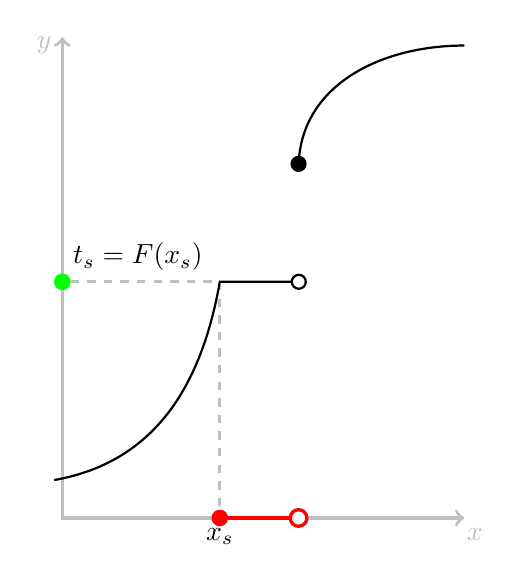
\begin{tikzpicture}[very thick,shorten >=-3pt,shorten <=-3pt]
	%\coordinate (A1) at (0,0);
	%\coordinate (A2) at (10,10);
	%\draw [help lines, lightgray] (A1) grid (A2);

	\draw [<->, lightgray] (0, 6) -- (0, 0) -- (5, 0);
	\node [left, lightgray] at (0,6) {$y$};
	\node [below right, lightgray] at (5,0) {$x$};

	\coordinate (x1) at (0,3);
	\coordinate (x2) at (2,3);
	\coordinate (x3) at (2,0);
	\coordinate (x4) at (3,3);

	\draw [->,dashed,lightgray] (x1) -- (x2) -- (x3);
	%% black line (CDF)
	\draw[thick,-o] (0,0.5) to [out=10,in=260] (x2) -- (x4);
	\draw[thick,*-] (3,4.5) to [out=90,in=180] (5,6);
	\node [above right] at (x1) {$t_s = F(x_s)$};
	\node [below] at (x3) {$x_s$};
	%\node [below right] at (x3) {$x_s = F^{-}(t_s)$};

        \draw[red] (2,0) -- (3,0);

        \fill[green] (x1) circle [radius=3pt];
        \fill[red] (x3) circle [radius=3pt];
        \draw[red,fill=white] (3,0) circle [radius=3pt];

\end{tikzpicture}

\end{document}
